\documentclass{article}
\usepackage[utf8]{inputenc}
%\usepackage[T2A]{fontenc}
\usepackage[russian]{babel}
\usepackage{siunitx}
\usepackage{csquotes}
\usepackage{url,amsmath,amssymb,fancybox,listings,pdfpages,caption,multicol,datetime,rotating, booktabs}
\usepackage{geometry}
\geometry{verbose,tmargin=1in,bmargin=1in,lmargin=1in,rmargin=1in}
\usepackage{graphicx}
\graphicspath{.}

\usepackage{svg}
\usepackage{shellesc}
\usepackage{subcaption}
\usepackage{float}

%opening
\title{Отчёт по работе на СТМ}
\author{Николаев Владислав\\
\texttt{v.nikolaev2@g.nsu.ru} \and
Матяш Алексей\\
\texttt{a.matyash@g.nru.ru}}
\date{22 сентября 2024 г.}

\begin{document}
\DeclareGraphicsExtensions{.jpg,.png,.gif,.svg}
\maketitle
\section{Теоретические основы}
Фундаментальный принцип работы:
\begin{figure}[h]

	\centering\includesvg[width=0.5\textwidth, keepaspectratio]{tunnelling}
\end{figure}

\begin{displayquote}
	The electrons can tunnel between two metals only from occupied states on one side into the unoccupied states of the other side of the barrier.
\end{displayquote}
Высокое разрешение обусловлено тем, что при небольшом увеличении $d$, ток туннелирования резко падает
$$I_t \approx U_t \times e^{-bd}$$


\begin{figure}[H]
	\centering
	\begin{subfigure}{0.49\textwidth}
		\centering
		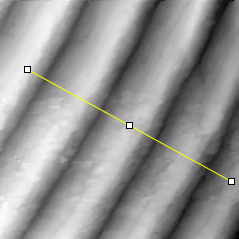
\includegraphics[width = \textwidth, keepaspectratio]{2789-1}
		\caption{Снимок}
		\label{fig:left}
	\end{subfigure}
	\begin{subfigure}{0.49\textwidth}
		\centering
		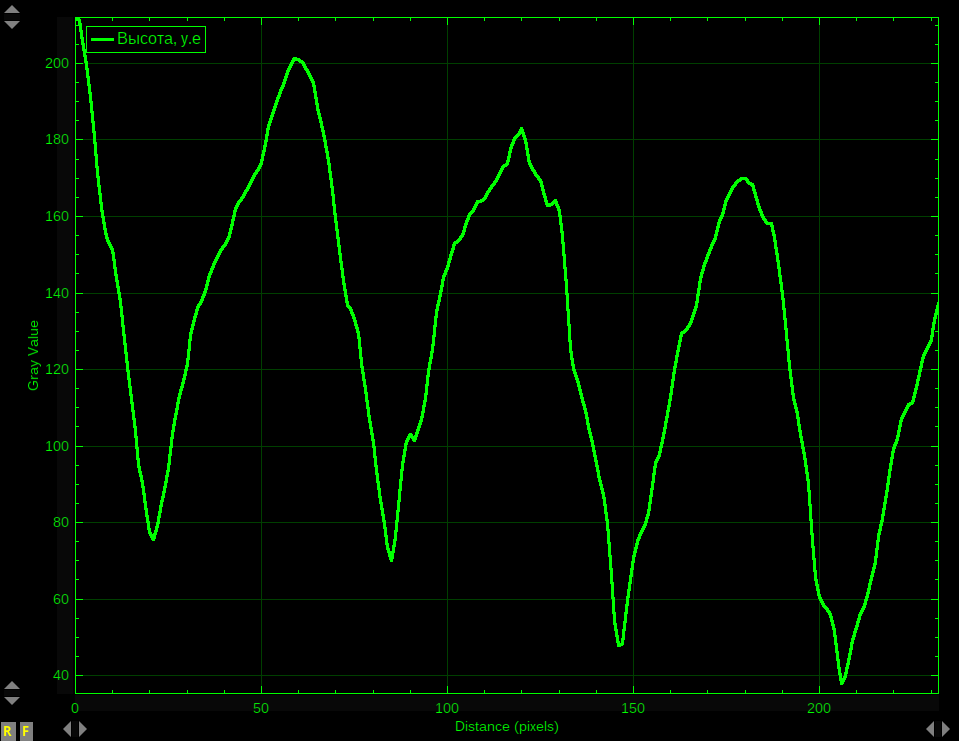
\includegraphics[width = \textwidth, height=8.09cm]{Plot of 2789}
		\caption{Профиль интенсивности по указанной линии}
		\label{fig:right}
	\end{subfigure}
	\caption{Снимок со стороной 2.789 \unit{\micro\meter}}
	\label{fig:combined}
\end{figure}
\section{Обработка результатов}
Для статистики замеряли ширину дорожки. Получили такие значения:
$$l=\{0.745, 0.741, 0.763, 0.760, 0.765\}, \unit{\micro\meter}$$

Статичтическая погрешность (стандартное отклонение) $0.01  \unit{\micro\meter}$.\\


Получили $l = 0.75 \pm 0.01\unit{\micro\meter}$.
Это согласуется с литературными данными, согласно которым  $l = 0.74 \unit{\micro\meter}$.\\

Предположительно, среднее завышено за счёт того, что защитный слой диска был удалён.

\section{Оценка объёма информации, которая может быть записана на диске}
Допустим, запись идёт в пределах от $r_{in}$ до $r_{ex}$, а ширина дорожки $l$.
Вычислим длину дорожки в приблежении, что она является спиралью.

В полярных координатах она задаётся как $(r,\phi)$. Притом $\phi=a\cdot r$. Хотим $\phi(r+l)=\phi(r)$. То есть за поворот на $2\pi$ $r$ увеличивается на l. То есть $$\frac{\phi}{2\pi}=\frac{r}{l}$$

$$r(\phi)=\frac{l}{2\pi}\phi$$
Длина кривой в полярных координатах задаётся выражением:
$$L = \int_{\phi_1}^{\phi_2} \sqrt{r^2(\phi) + {r'_\phi}^2}\,d\phi$$
Оценим $\phi_1$ и $\phi_2$:
$$\phi_1\approx \frac{(r_{in}-0)}{l}2\pi=\frac{(r_{in})}{l}2\pi$$
$$\phi_2\approx \frac{(r_{ex}-r_{in})}{l}2\pi$$
По данным из интернета:
$$r_{in}=7.5\unit{\milli\meter}=7.5\cdot 10^3\unit{\micro\meter}$$
$$r_{ex}=60\unit{\milli\meter}=6.0\cdot10^4\unit{\micro\meter}$$

Однако есть нюанс: $r_{ex}$ здесь радиус именно отверстия, поэтому запись данных начинается от большего радиуса, но для оценки сверху подойдёт.\\

Таким образом численно:
$$\phi_1\approx 6.37\cdot10^4 \unit{\radian}$$
$$\phi_2\approx 4.46\cdot10^5 \unit{\radian}$$

Подставим в подынтегральное выражение $r$ и $r'$:
$$\sqrt{r^2(\phi) + {r'_\phi}^2} = \sqrt{\left(\frac{l}{2\pi}\right)^2\phi^2+\left(\frac{l}{2\pi}\right)^2} = \frac{l}{2\pi} \sqrt{\phi^2+1}$$
Наконец проинтегрируем:
\begin{equation}
\begin{split}
	L &= \frac{l}{2\pi}\int_{\phi_{1}}^{\phi_2} \sqrt{\phi^2+1}\,d\phi \\
	&= \frac{l}{2\cdot 2\pi}\left(\phi\sqrt{1+\phi^2}+\ln \left|\phi+\sqrt{1+\phi^2}\right|\right)\Biggr|_{\phi_1}^{\phi_2} \\
	&= \frac{0.74}{2\cdot 2\pi}\left(1.99\cdot10^{11}-4.06\cdot10^{9}\right)\\
	&= 1.15 \cdot 10^{10}\unit{\micro\meter}
\end{split}
\end{equation}
Считаем, что 1 бит занимает $l$ длины спирали, тогда всего на диске помещается $$I=\frac{L}{l} = 1.55\cdot10^{10}\unit{\bit}=1.8\unit{\giga\byte}$$
Это немного меньше, чем действительный объём диска, который составляет $4.7\unit{\giga\byte}$.\\
По литературным (интернетным) данным длина бита $130\unit{\nano\meter}=0.13 \unit{\micro\meter}$. Так получается, что объём диска $10.3\unit{\giga\byte}$. Видимо, эти данные не учитывают пустое место внутри дорожки, потому что результат отличается примерно в два раза от реальности.
\end{document}
